\documentclass{beamer}

% for themes, etc.
\mode<presentation>{ 
\usetheme{Rochester} 
}

\usepackage{graphicx}
\usepackage{tikz}
\usetikzlibrary{shapes, arrows, positioning}

\title[]{A Surrogate Approach Towards Validation and Uncertainty Quantification of Multiphysics Reactor Simulation Codes}
\subtitle[]{Thesis Prospectus}
\author[]{Artem Yankov}
\institute[]{University of Michigan}
\date{April 17, 2014}

% have this if you'd like a recurring outline
\AtBeginSection[]  % "Beamer, do the following at the start of every section"
{
\begin{frame}<beamer> 
\frametitle{Outline} % make a frame titled "Outline"
\tableofcontents[currentsection]  % show TOC and highlight current section
\end{frame}
}

\begin{document}

% this prints title, author etc. info from above
\begin{frame}
\titlepage
\end{frame}

% MOTIVATION
\section{Motivation}

%%%%%%%%%%%%%%%%%%%%%%%%%%%%%%%%%%%%%%%%%%%%%%%%%%%%%%%%%%%%%%%%%%%%%%%%%%%%%%%%%%%%%%%%
\begin{frame}
\frametitle{Background}

\begin{itemize}
  \item Physical phenomena is studied by conducting experiments. 
  \item Any data collected represents instances of underlying stochastic processes.  
  \item We build predictive computer models in an attempt to reproduce such observed physical phenomena.
  \item To accurately capture stochastic element of experiments, computer models should be probabilistic.  
  \item In other words, inputs to computer models have uncertainties associated with them that are propagated to any outputs of interest.
  \item Running computer simulations should be like conducting physical experiments. Computer experiments.      
\end{itemize}

\end{frame}
%%%%%%%%%%%%%%%%%%%%%%%%%%%%%%%%%%%%%%%%%%%%%%%%%%%%%%%%%%%%%%%%%%%%%%%%%%%%%%%%%%%%%%%%
\begin{frame}
\frametitle{Why Surrogates?}

\begin{itemize}
  \item We run computer simulations to meet design objectives under certain constraints. 
  \item Involves numerical optimization, calibration, and performing what-if analyses.
  \item Also, we're interested in determining which of our design variables have the greatest effects on simulation outcomes. 
  \item Thousands of simulations required to make this possible but...  
  \item Computer simulations that model real phenomenon like nuclear reactors often take $\mathcal{O}(\mbox{hours})$ or $\mathcal{O}(\mbox{days})$ to complete.
  \item Building a surrogate model for your expensive computer simulations can make everything listed above possible.   
\end{itemize}

\end{frame}
%%%%%%%%%%%%%%%%%%%%%%%%%%%%%%%%%%%%%%%%%%%%%%%%%%%%%%%%%%%%%%%%%%%%%%%%%%%%%%%%%%%%%%%%
\begin{frame}
\frametitle{What is a Surrogate Model?}

\begin{itemize}
  \item A model for the outcomes of (likely) expensive computer simulations that can be rapidly evaluated while simultaneously preserving the predictive capabilities of the original simulations.
  \item Want to intelligently choose subspace $\lbrace x_1, x_2, ..., x_N\rbrace \subset \mathbf{X}$ to sample expensive computer code to get $\lbrace y_1, y_2, ..., y_N\rbrace \subset \mathbf{Y}$.
  \item Learn fast mapping that approximates $\mathbf{X}\rightarrow\mathbf{Y}$.   
\end{itemize}

\begin{figure}
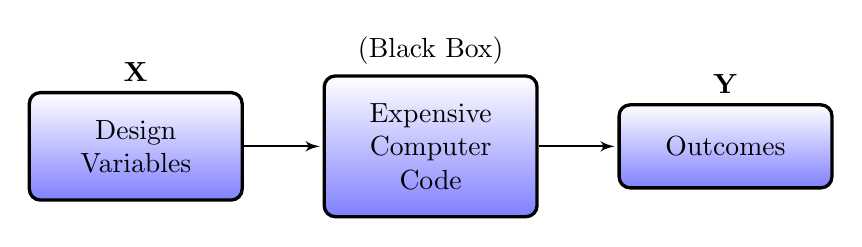
\begin{tikzpicture}[node distance=1cm, auto]  
\tikzset{
    mynode/.style={rectangle,rounded corners,draw=black, top color=white, bottom color=blue!50,very thick, inner sep=1em, minimum size=3em, text centered},
    myarrow/.style={->, >=latex', shorten >=1pt, thick},
    mylabel/.style={text width=7em, text centered} 
}  
\node[mynode, text width=2cm, label=$\mathbf{X}$] (design_vars) {Design Variables};  
\node[mynode, right= of design_vars, text width=2cm, label=(Black Box)] (computer_code) {Expensive Computer Code};
\node[mynode, right= of computer_code, text width=2cm, label=$\mathbf{Y}$] (outcomes) {Outcomes};
\draw[myarrow] (design_vars) edge node {} (computer_code);
\draw[myarrow] (computer_code) edge node {} (outcomes);
\end{tikzpicture}  
\end{figure}

\end{frame}

% PROPOSED APPLICATION
\subsection{Proposed Application}
%%%%%%%%%%%%%%%%%%%%%%%%%%%%%%%%%%%%%%%%%%%%%%%%%%%%%%%%%%%%%%%%%%%%%%%%%%%%%%%%%%%%%%%%
\begin{frame}
\frametitle{Proposed Application to Fuel Performance Modeling}

\begin{itemize}
  \item Fission Gas Release (FGR) refers to the phenomenon where Xenon and Krypton gases formed in UO$_2$ fuel rods are released into the rod filling gas.
  \item Causes pressure build-up and thermal conductivity degradation in the rod filling gas, potentially jeopardizing the safety of the reactor.
  \item Fission gas atoms generated in the fuel grains diffuse towards the grain boundaries. 
  \item Majority of the gas diffuses into grain-face gas bubbles, giving rise to grain-face swelling.
  \item Bubble growth brings about bubble coalescence and interconnection, eventually leading to the formation of a tunnel network through which the fission gas is released.       
\end{itemize}

\end{frame}   
%%%%%%%%%%%%%%%%%%%%%%%%%%%%%%%%%%%%%%%%%%%%%%%%%%%%%%%%%%%%%%%%%%%%%%%%%%%%%%%%%%%%%%%%
\begin{frame}
\frametitle{SIFGRS FGR Model}

\begin{itemize}
  \item Simple Integrated Fission Gas Release and Swelling (SIFGRS)
  \item Incorporates gas diffusion and precipitation in grains, growth and coalescence of gas bubbles at grain faces, thermal, athermal, steady-state, and transient gas release. 
  \item Through a direct description of the grain face gas bubble development, the fission gas swelling and release are calculated as coupled processes.
  \item Parameterized by, among others, linear heat rate, gas diffusion coefficient, surface tension of grain face bubbles, hydrostatic pressure, fuel grain radius, fuel porosity, and grain boundary sweeping. 
\end{itemize}

\end{frame}
%%%%%%%%%%%%%%%%%%%%%%%%%%%%%%%%%%%%%%%%%%%%%%%%%%%%%%%%%%%%%%%%%%%%%%%%%%%%%%%%%%%%%%%%
\begin{frame}
\frametitle{Ris\o~AN3 Experiment}

\begin{itemize}
  \item Validation case for fuel performance modeling in the Fumex-II database.
  \item Experiment consists of a base irradiation of four reactor cycles in the Biblis A pressurized water reactor.
  \item After the base irradiation period, a fuel rod is extracted and refabricated to a shorter length before undergoing a power ramp.
  \item Refabricated fuel rod is outfitted with various instrumentation such that fuel centerline temperature, FGR and rod internal pressure measurements can be obtained.    
\end{itemize}

\end{frame}
%%%%%%%%%%%%%%%%%%%%%%%%%%%%%%%%%%%%%%%%%%%%%%%%%%%%%%%%%%%%%%%%%%%%%%%%%%%%%%%%%%%%%%%%
\begin{frame}
\frametitle{Ris\o~AN3 Experiment Irradiation Profiles}

\begin{columns}
 \begin{column}{0.5\textwidth}
  \centering
  Base Irradiation History
  \includegraphics[width=1.\textwidth]{./base_irrad.png}
 \end{column}
 \begin{column}{0.5\textwidth}
  \centering
  Power Ramp Experiment
  \includegraphics[width=1.\textwidth]{./power_ramp.png}
 \end{column}
\end{columns}

\end{frame}
%%%%%%%%%%%%%%%%%%%%%%%%%%%%%%%%%%%%%%%%%%%%%%%%%%%%%%%%%%%%%%%%%%%%%%%%%%%%%%%%%%%%%%%%
\begin{frame}
\frametitle{Modeling Ris\o~AN3 Experiment with BISON}

\begin{itemize}
  \item BISON is a finite-element fuel performance modeling code that utilizes the SIFGRS model.
  \item SIFGRS parameters are quite generic and uncertain. 
\end{itemize}

\begin{columns}
 \begin{column}{0.5\textwidth}
  \centering
  Fission Gas Release
  \includegraphics[width=1.\textwidth]{./fgr_comparison.png}
 \end{column}
 \begin{column}{0.5\textwidth}
  \centering
  Fuel Centerline Temperature
  \includegraphics[width=1.\textwidth]{./tc_temp_comparison.png}
 \end{column}
\end{columns}

\end{frame}
%%%%%%%%%%%%%%%%%%%%%%%%%%%%%%%%%%%%%%%%%%%%%%%%%%%%%%%%%%%%%%%%%%%%%%%%%%%%%%%%%%%%%%%%
\begin{frame}
\frametitle{Modeling Ris\o~AN3 Experiment with BISON/MPACT}

\begin{itemize}
  \item No sense in comparing the output of a computer simulation to
experimental data unless the computer simulation is of high fidelity and capable
of reproducing the pertinent physics.
  \item MPACT is a neutronics code that provides detailed intrapin and azimuthally dependent
neutronics data in the fuel elements. 
  \item The two-way coupling scheme provided by BISON and MPACT provides the most accurate fuel performance modeling available for a nuclear reactor.
  \item Expensive! 
\end{itemize}

\end{frame}
%%%%%%%%%%%%%%%%%%%%%%%%%%%%%%%%%%%%%%%%%%%%%%%%%%%%%%%%%%%%%%%%%%%%%%%%%%%%%%%%%%%%%%%%
\begin{frame}
\frametitle{Modeling Ris\o~AN3 Experiment with BISON/MPACT}

\begin{itemize}
  \item BISON predictions of FGR and temperature fields stand to be improved by calibrating FGR parameters to experimental data.
  \item Calibration studies require $\mathcal{O}(10^3)$ function evaluations, which in this case are the coupled BISON/MPACT computer codes.
  \item Each simulation of the Ris\o~AN3 experiment will take a few hours.
  \item It's necessary to construct a surrogate for the calibration study!   
\end{itemize}

\end{frame}
%%%%%%%%%%%%%%%%%%%%%%%%%%%%%%%%%%%%%%%%%%%%%%%%%%%%%%%%%%%%%%%%%%%%%%%%%%%%%%%%%%%%%%%%

% SURROGATE CONSTRUCTION
\section{Building Surrogate Models}

% APPLICATION OF SURROGATE METHODS
\section{Application of Surrogate Models}




\end{document}